\documentclass{article}
\usepackage{blindtext}
\usepackage{tcolorbox}
\usepackage{graphicx}
\usepackage[top=2cm, bottom=2cm, outer=0cm, inner=0cm]{geometry}
\usepackage[pages=some]{background}
\usepackage[paper=portrait,pagesize]{typearea}
\usepackage[utf8]{inputenc}
\setlength{\arrayrulewidth}{0.5mm}
\setlength{\tabcolsep}{18pt}
\renewcommand{\arraystretch}{1.5}

\begin{document}

\KOMAoptions{paper=landscape,pagesize}
\backgroundsetup{
	scale=1,
	color=black,
	opacity=10,
	angle=0,
	contents={%
		
\includegraphics[width=\paperwidth,height=\paperheight]{Picture3.jpg}
	}%
}

\begin{tcolorbox}[width=\textwidth,colback={blue},outer arc=0mm,colupper=white]    
\huge \textbf{THE HISTORICAL PERSPECTIVE OF PYTHON, HTML, CSS, JAVA AND C++} 


\small BY GINA CAPTAIN-BRIGGS
	
\end{tcolorbox} 
\BgThispage
\noindent{%
	
	\parbox{\textwidth}{%
		
	}%

	
	\newpage
	
\huge \centering The highlights of each Programming language:
	\begin{tcolorbox}[width=\textwidth,colback={teal},outer arc=0mm,colupper=white]    
		\huge History
	\end{tcolorbox} 
\begin{tcolorbox}[width=\textwidth,colback={cyan},outer arc=0mm,colupper=white]    
	\huge Founder
\end{tcolorbox} 
\begin{tcolorbox}[width=\textwidth,colback={gray
	},outer arc=0mm,colupper=white]    
	\huge Application examples that exist or can be developed
	
	
\end{tcolorbox} 
\begin{tcolorbox}[width=\textwidth,colback={lime},outer arc=0mm,colupper=white]    
	\huge \textbf{Available Integrated Development Environment (IDEs) you can use}
	
\end{tcolorbox}
\begin{tcolorbox}[width=\textwidth,colback={green},outer arc=0mm,colupper=white]    
	\huge Related programming languages
	
\end{tcolorbox} 
	\newpage
	
\includegraphics[width=\linewidth,height=\linewidth]{Picture4.png}
\centering
\begin{tcolorbox}[width=\linewidth,colback={blue},outer arc=0mm,colupper=white]    
	\huge PYTHON
	
\end{tcolorbox} 
	\newpage

History
In 1980, Python was created by Guido van Rossum at Centrum Wiskunde and Informatica (CWI) within the Netherlands. 
Its execution began in 1989.
Founder
Guido van Rossum
Application examples
Developing games
AI and machine learning. 
Information analytics.
Information visualization. 
Programming applications. 
Internet development. 
Language development. 
Finance.
Available Integrated Development Environment (IDEs) 
IDLE (Integrated Development and Learning Environment)
PyCharm
Visual Studio Code. 
Sublime Text 3. 
Atom. 
Jupyter. 
Spyder. 
PyDev.

Related programming languages
Java, JavaScript, Perl, Tcl, Smalltalk

\newpage

\includegraphics[width=\linewidth,height=\linewidth]{Picture1.png}
\centering
\begin{tcolorbox}[width=\linewidth,colback={blue},outer arc=0mm,colupper=white]    
	\huge HTML
\end{tcolorbox} 

\newpage
History
In 1991, hypertext mark-up language was designed by Tim Berners-Lee.
In 1993, HTML 1.0 was released to assist with sharing info that may be legible and accessible through internet browsers on the web.
In 1995, it had been revealed as HTML 2.0
In 1999, a significant version of hypertext mark-up language, HTML 4.01 was revealed.
Founder
Tim Berners-Lee
Application examples
In developing web content
Making numerous internet documents
Navigating the internet
It helps with entering Data
Developing games
Available Integrated Development Environment (IDEs) 
Atom
Komodo Edit
WebStorm
PhpStorm
Light Table
Codelobster
Rapid PHP Editor
PHP Development
Adobe Dreamweaver

Related programming languages
XHTML

\newpage

\includegraphics[width=\linewidth,height=\linewidth]{Picture2.png}
\centering
\begin{tcolorbox}[width=\linewidth,colback={blue},outer arc=0mm,colupper=white]    
	\huge CSS
\end{tcolorbox} 

\newpage
History
October 10, 1994, CSS was planned by Hakon Wium Lie who was operating with Tim Berners-Lee at CERN at the time.
It had been developed to produce style sheets for the web.
It had been developed by the World Wide Web Consortium (W3C).
Founder
Hakon Wium Lie
Application examples
End-User and Server-Side Representation
E-Commerce Domain
Website Maintenance
Handling Flash Animation and effects
Handling dynamic Website Templates

Available Integrated Development Environment (IDEs) 

Brackets
Atom
PyCharm
Visual Studio Code
PhpStorm
NetBeans
WebStorm
Komodo Edit
Related programming languages
Sass, Bootstrap, JavaScript, Python, Ruby

\newpage

\includegraphics[width=\linewidth,height=\linewidth]{Picture3.png}
\centering
\begin{tcolorbox}[width=\linewidth,colback={blue},outer arc=0mm,colupper=white]    
	\huge JAVA
\end{tcolorbox} 

\newpage
History
In 1995, Java was created by James Gosling. James Gosling and his team members started the project within the early ‘90s.
Founder
James Gosling
Application examples
Internet programming
Solutions to e-businesses
Mobile devices and their applications
Games
Science
Enterprises
Desktop GUI
Available Integrated Development Environment (IDEs) 
JBuilder
Code::Blocks
WebStorm
Visual Studio Code

Related programming languages
Smalltalk, Lisp

\newpage
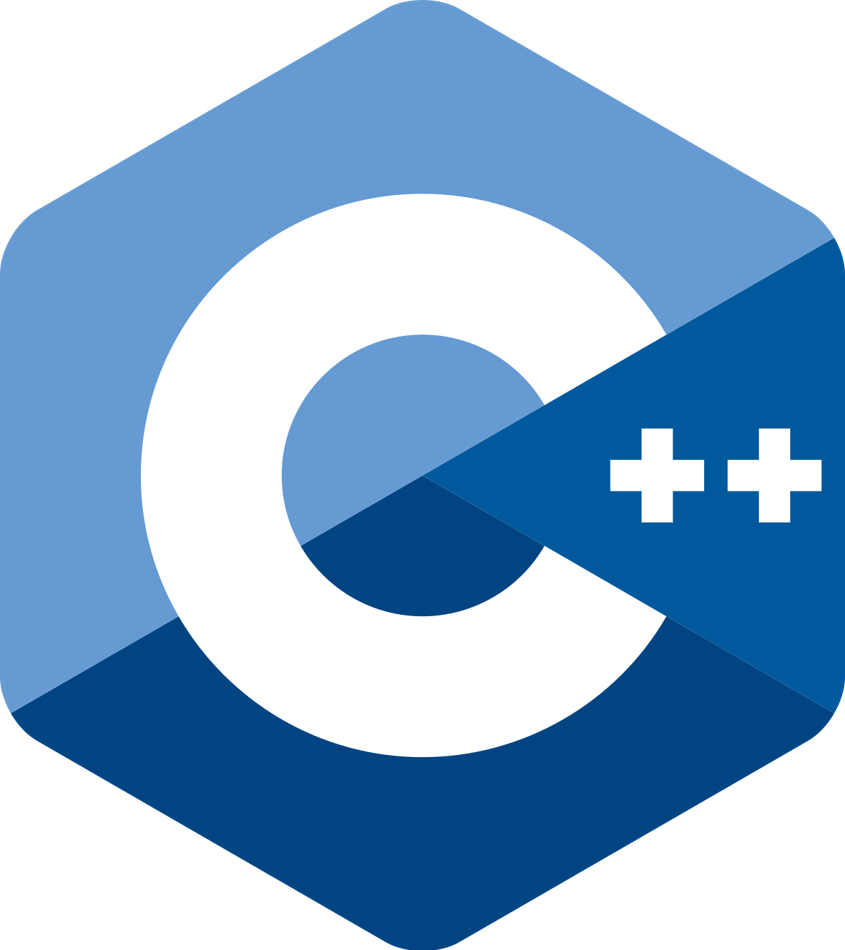
\includegraphics[width=\linewidth,height=\linewidth]{Picture5.png}
\centering
\begin{tcolorbox}[width=\linewidth,colback={blue},outer arc=0mm,colupper=white]    
	\huge C++
\end{tcolorbox} 

\newpage
History
In 1979, C++ started being developed by Bjarne Stroustrup at Bell Laboratories.
Earlier it had been known as  “C with Objects” as a result of C++ being a trial to feature object-oriented options and different enhancements to C.
In 1983, as the language developed, Stroustrup named it C++. 
Founder
Bjarne Stroustrup
Application examples
In Operation Systems
Browsers
Games
Advanced Graphics and Computation
Cloud systems
Banking Applications

Available Integrated Development Environment (IDEs) 
Code::Blocks
Microsoft Visual Studio
Eclipse
Kdevelop
C++Builder
NetBeans
Clion
CodeLite
XCode
Atom
Microsoft Visual Code
Related programming languages
Java
Python
Ruby



\newpage
THANK YOU!

\end{document}
